\documentclass[output=paper]{LSP/langsci} 
\ChapterDOI{10.5281/zenodo.1090972}
\author{Mario Bisiada\affiliation{Universitat Pompeu Fabra}}
\title{Universals of editing and translation}
\abstract{%
  It has been claimed that translation universals are really \enquote{mediation universals} \parencites{chesterman04}{ulrmur08}, pertaining to the more general cognitive activity of mediating a text rather than specifically translating it. Among those linguistic activities that share the alleged mediation effect with translating are editing and revising. In this chapter, I critically examine the theory of \enquote{mediation universals} by comparing unedited translations with edited translations and with edited non-translations. The focus is on explicitation, normalisation\slash conservatism and simplification. The operationalisations are partly adopted from a similar study on English by \textcite{kruger12}, which the present study seeks to replicate for German management and business articles. The results do not support the notion of mediation universals for the present corpus but rather show that translated texts are recognisable as such even after the editing process. Editorial influence on translated language in this genre is shown to be strongest in terms of sentence length and lexical diversity, where unedited and edited translations differ significantly from each other. Here, editors approximate the language to that of the non-translations, though the unedited translations have a greater average sentence length than the non-translations. That finding does not support the usual observation that translated texts have shorter sentences than non-translations, but highlights the importance of studying editorial influence in translation. That translations are hybrid texts, influenced by many agents other than the translator is now trivial knowledge. Yet corpus research in translation studies still relies mainly on published translations. The findings in this chapter argue for including unedited manuscripts in corpus-based studies of translated language to avoid missing phenomena of translated language that may be removed at the editing stage and to be able to differentiate which features really pertain to the translation act and which are affected by editorial influence.
}

\maketitle

\begin{document}

\section{Introduction}

The notion of translation \isi{universals} has been subject to debate for a long time \parencites{baker93}{chesterman04}{mauranen04}. Its status today is problematic \parencite[see][]{house08}, though few would dispute that differences exist between translated and non-translated texts. Much of the controversy surrounding the issue is about the term \enquote{universal} \parencite[86]{chesterman14}, while the line of enquiry itself still seems productive and interesting because ``the quest for \isi{universals} is no more than the usual search for patterns and generalizations that guides empirical research in general'' \citep[87]{chesterman14}.

To advance translation studies as an empirical discipline, it is necessary to test existing theories with empirical methods and to suggest new models based on empirically tested (and testable) data. This process can be facilitated by conceiving studies in a replicable and rigorously transparent fashion, that is, they should enable other researchers to retrace the steps taken by the investigator, so that they can test the results in another language, genre or setting. To promote the use of statistical significance testing in our discipline, it would be useful for scholars to cite the sources where the significance tests they employ are documented, just as it is done with other tools or ideas that they use in their work. Merely stating the name of a statistical test without reference assumes that it is common knowledge, which in many disciplines of the humanities is arguably not the case.

The aim of this chapter is to draw attention to the influence of editors on the translation text, which so far has not received much attention in models of translation. Studying texts before and after \isi{editing} can provide great insights into the \isi{translation process}, which is here defined as ``the period commencing from the moment the client contacts the translator and ending when the translation reaches the addressee'' \citep[179]{munoz10}.

Most analyses of translated language are based solely on corpora of published translations, and few attempts have been made to build a corpus of unedited translations \parencite[for an early such design, see][]{utka04}. But published texts have usually undergone some kind of \isi{editing} process involving various language users prior to their release. The study of manuscript translations informs current theories of translation by differentiating linguistic features that are present throughout the \isi{translation process} from features whose frequency in the text was increased or decreased at the \isi{editing} stage.

A holistic view of the \isi{translation process}, obtained by studying manuscript translations alongside their published versions, will greatly increase the accuracy of the claims we make about translated language, improve the \enquote{ecological validity of experimental settings} \parencites[179]{munoz10}[see also][110]{salobr13}, and allow insights into the linguistic effects of \isi{editing}, an as yet underresearched aspect of language use \parencites{bisiada17tr}{bisiada17pst}.

This chapter investigates three proposed translation \isi{universals}, \isi{explicitation}, normalisation and simplification, aiming to find out how these are affected by editorial intervention. Those \isi{universals} were chosen in order to allow a comparison of results to those found by \textcite{kruger12}. Partly adopting her methodology, I compare two subcorpora that each exhibit one type of \isi{mediation} (one translated but not edited, the other not translated but edited) with a third subcorpus that exhibits both types of \isi{mediation}, that is, the texts were translated and then edited.

If translating and \isi{editing} really are a comparable type of language use and could be subsumed under the label of \enquote{mediation}, there should be little to no differences between manuscript and published translations, because the translation stage should already have applied the \enquote{\isi{mediation} universals}. The published translations should then also be rather similar to the published non-translations, as both have undergone the \isi{editing} process.

A more likely scenario seems to be that the texts differ with respect to particular \isi{universals} but not to others. Tracing the evolution of the translated texts through the translation and \isi{editing} stage will thus give us an idea of what stage tends to affect which type of universal. It will also allow us to investigate whether \isi{editing} leads to a similar product when it takes place on non-translated compared to translated texts, as, for instance, editors aim to assimilate translated language to that found elsewhere in their publication.

The chapter is structured as follows: Section~\ref{bisiada:sec:lit} discusses existing claims that translation \isi{universals} are really \enquote{\isi{mediation} universals}. In Section~\ref{bisiada:sec:corp}, I describe the corpus and the operationalisations of the three translation \isi{universals} that were tested in this study. I then explain the statistical methods used and the procedure that I took to ensure statistical significance of the findings (Section~\ref{bisiada:sec:statsig}). Section~\ref{bisiada:sec:anal} contains the analysis of \isi{explicitation} (\ref{bisiada:sec:expl}), normalisation\slash conservatism (\ref{bisiada:sec:norm}) and simplification (\ref{bisiada:sec:simp}). Finally, Section~\ref{bisiada:sec:disc} contains a summary of the findings and a discussion of their implications.

\section{Universals of \enquote{mediated discourse}?}\label{bisiada:sec:lit}

Translating and \isi{editing} are considered to be forms of \isi{mediation}. \citeauthor{lefevere92} argues that what translating has in common with \enquote{other modes of rewriting, such as \isi{editing}, historiography, criticism, anthologising and the production of abridged or simplified texts} is that it \textcquote[9]{lefevere92}{presuppose[s] a certain degree of \isi{mediation} on the part of the writer\slash translator to adapt texts to the new audience}.

In his analysis of translation \isi{universals}, \textcite{chesterman04} calls translation an act of \enquote{constrained communication}, arguing that \isi{universals} pertinent to translation may also be found ``in other kinds of constrained communication, such as communicating in a non-native language or under special channel restrictions, or any form of communication that involves relaying messages, such as reporting discourse, even journalism.'' \citep[10--11]{chesterman04} Crucially, he argues that ``it may be problematic eventually to differentiate factors that are pertinent to translation in particular from those that are pertinent to constrained communication in general'' \citep[10--11]{chesterman04}. This view was already held by \textcite[21]{BlumKulka1986} concerning the proposed universal of \isi{explicitation}, which, she argues, \enquote{might be [\ldots] a universal strategy inherent in the process of language \isi{mediation}, as practiced by language learners, non-professional translators and professional translators alike}.

\textcite{ulrmur08} adopt the notion of \enquote{constrained communication} and the list of linguistic activities that are claimed to share particular features, so-called \enquote{\isi{mediation} universals} \parencite*[149]{ulrmur08}. They even add to that category by arguing that \enquote{\isi{editing}, copy-\isi{editing}, \isi{revision} or postediting} as well as ghost-writing are also types of mediated discourse \parencite*[150]{ulrmur08}. What unites texts of that kind, in their view, is that \textcquote[151]{ulrmur08}{they are processed, or rewritten, for particular audiences and are thus mediated for a purpose}. Like \citeauthor{chesterman04}, they argue that ``the notion of translation \isi{universals} may be usefully replaced by that of \emph{\isi{mediation} universals} which may be identified in various kinds of mediated discourse'' \citep[149]{ulrmur08}. 

By the above definition, most publicly available texts, except perhaps spontaneous online discourse such as comments, posts or tweets, could be described as \enquote{mediated discourse}. Such a wide applicability not only makes the term itself less useful. It also makes the hypothesis of \enquote{\isi{mediation} universals} difficult to disprove, as very few texts are available that would be considered \enquote{unmediated discourse}. Internet discourse might be one possibility, but one would have to ensure that the authors are native speakers, have not reported any discourse or relayed any messages and have not revised their text. The reliability of such a corpus would seem to be rather low.

To back up their claims, \textcite{ulrmur08} conduct a study of mediated discourse, where they draw on the EuroCom corpus, a parallel corpus of written texts drafted by non-native speakers of English at the European Commission and the same texts edited by native speakers. The size of the corpus at the time of analysis is reported as one million words in each part of the corpus \parencite[152]{ulrmur08}. The object of study is to investigate \textcquote[155]{ulrmur08}{whether there are typical phraseologies within mediated discourse as such} by comparing the edited texts both with the non-edited texts in the corpus and with the British National Corpus (BNC), which they call \textcquote[155]{ulrmur08}{a corpus of non-mediated native-speaker language}.

Analysing three-word clusters, they find that \emph{in order to} and \emph{as well as} are used rather often in the EuroCom corpus, though more commonly in the non-edited than in the edited texts. Further, they are used less often in the BNC, from which they conclude that \textcquote[159]{ulrmur08}{they are not used frequently in speech or writing in non-mediated English}.

However, these findings do not seem very convincing. As a \textcquote[159]{ulrmur08}{reference corpus of native-speaker, non-mediated English}, the BNC may be problematic. It contains extracts from, among other things, national newspapers, specialist periodicals, academic books, popular fiction and university essays, the authors of which are unlikely to be native speakers in all cases. And even if that were the case, a claim that is not made anywhere in the description of the BNC \parencite{bnc09}, the corpus does not seem to contain much \enquote{non-mediated} English. It does contain some unpublished letters and essays that may be considered non-edited, and thus non-mediated. But for the most part, it consists of published, and thus mediated, texts, as newspapers, periodicals, journals and books have all been edited, copy-edited and revised to some extent.

Elsewhere, \textcite{ulrych09} claims that the boundaries between translating and \isi{editing} as forms of \isi{mediation} are becoming blurred. Unfortunately, it is not clear just what is meant by \isi{editing}, specifically who does the \isi{editing}. The research approach taken by \textcite{ulrmur08} outlined above suggests that the \isi{editing} is done by someone other than the translator. However, the reference to \textcquote[219]{ulrych09}{hybrid forms such as transediting} seems to suggest that it is the authors or translators themselves who do the \isi{editing} \parencite[for a valuable critique of the term \enquote{transediting}, see][]{schäffner12}.

The existence of \enquote{\isi{mediation} universals}, then, has never really been substantiated by empirical evidence. That has not kept it from being used, albeit with different understandings: to refer to non-native speaker language use \parencites{ulrans08}{gasber10}[79]{rabizq13}[175]{xiahu15}, to bilingual communication \parencite{lanhel12}, to interlingual \isi{revision} \parencite[63]{robertson10} or to \textcquote[183]{zanettin14}{texts produced under the constraint of linguistic or cultural contact}. Even the term \enquote{mediation} itself is used without a commonly accepted definition \parencites[for a totally unrelated use of the term \enquote{mediated discourse}, see][]{scollon01}{norjon05}.

One empirical analysis of \enquote{\isi{mediation} universals} and, more specifically, the \isi{mediation} effect of \isi{editing}, was conducted by \textcite{kruger12}. The 1.2 million word corpus she draws on has three subcorpora: firstly, translations from \ili{Afrikaans} to English, secondly, originally English texts that were edited by professional language editors, and thirdly, those same texts in their manuscript form before \isi{editing} took place \parencite*[360]{kruger12}. All texts are from the time span 1997 to 2010 and the genres are academic, instructional, popular and reportage texts \parencite*[359]{kruger12}. Her aim is to investigate whether ``the \isi{universals} of translated language are the consequence of a cognitive \isi{mediation} effect that is shared among different kinds of mediated language'' \citep[358]{kruger12}. Her analysis focuses on the three suggested translation \isi{universals} \isi{explicitation}, normalisation\slash conservatism and simplification (more details on the operationalisations she uses to study these \isi{universals} are given in Section~\ref{bisiada:sec:meth}).

Her findings do not support the hypothesis that translation \isi{universals} are really \isi{mediation} \isi{universals} as there is a \enquote{consistent difference between the translated and edited subcorpus} in each of the three types of \isi{universals} investigated \parencite[380]{kruger12}. Instead, she argues that the differences she finds between the two corpora can be attributed to either of the facts that they differ in processing (monolingual vs bilingual) and in production circumstances (free vs constrained) \parencite[381]{kruger12}. She also suggests that \isi{editing} as a form of \isi{mediation} does not involve \isi{explicitation} or simplification, at least not as much as in translation, which she explains by the fact that \isi{editing} does not involve the production of a new text \parencite*[382]{kruger12}.

Translating and \isi{editing} also differ in that translating may to a larger extent be guided by the tendency of risk aversion \parencites{pym05}{pym08} than \isi{editing}, because translators produce a text while editors work on an existing text. The linguistic \isi{mediation} that translators undertake and which tends to make them \textcquote[20]{becher10}{avoid misunderstandings at all costs} is different to the \isi{mediation} entailed by the act of \isi{editing}, as it is either the translator or the author that will be blamed in case of communication problems. Universals affected by risk aversion are thus more likely to surface during the translation act than at the \isi{editing} stage.

On top of that, translators are often pressed for time and paid by the hour, working on several jobs at the same time, while the editors tend to be in-house employees (that is true at least for the editors who worked on the data in my corpus). Editors have told me that the quality of the translation is an important factor affecting the time they spend on an article, though different concepts of what exactly is \enquote{quality} in translation exist \parencites{drugan13}{mossop14}{house15tq}. Thus, the different production circumstances further argue against the existence of \enquote{\isi{mediation} universals}.

%%%%%%%%%%%%%%%%%%%%%%%%%%%%%%%%%%%%%%%%%%%%%%%%%%%%%%%%%%%%%%%%%%%%%%%%%%%%%%%%%%%%%
\section{Methodology}\label{bisiada:sec:meth}
%%%%%%%%%%%%%%%%%%%%%%%%%%%%%%%%%%%%%%%%%%%%%%%%%%%%%%%%%%%%%%%%%%%%%%%%%%%%%%%%%%%%%

\subsection{Corpus details and operationalisations}\label{bisiada:sec:corp}

The present study draws on a 300,000 word corpus of management articles with three subcorpora (detailed in Table~\ref{bisiada:tab:corpus}). The translated subcorpus (TR) consists of manuscript translations into \ili{German} of English articles that originally appeared in the \emph{Harvard Business Review}, an American magazine for business leaders and managers. The manuscript translations were provided to me by Rheinschrift, a translation company funded in 1995 and based in Cologne. These articles were translated by a range of translators and date from 2006 to 2011 and were commissioned by the \emph{Harvard Business Manager}, the \ili{German} sister publication of the \emph{Harvard Business Review}. The texts are drafts that were checked for accuracy within the translation company and then sent to the publisher for \isi{editing}.

\begin{table}
  \caption{Corpus details}\label{bisiada:tab:corpus}
  \begin{tabular}{lcccr}
    \lsptoprule
    Subcorpus& Translated?  & Edited?  & Texts (n)  & Size (words)\\
    \midrule
    TR      & yes       & no          & 27            & 106,829\\
    TR+ED   & yes       & yes         & 27            & 104,448\\
    ED      & no        & yes         & 27            & 88,312\\
    \lspbottomrule
  \end{tabular}
\end{table}

\noindent The subcorpus of translated and edited texts (TR+ED) consists of the edited and published versions of the translations in the TR subcorpus. The edited (ED) subcorpus consists of articles that were written by a range of authors for the \emph{Harvard Business Manager}, edited and published there in 2008. For the analysis, the three subcorpora were part-of-speech tagged and lemmatised using TreeTagger \parencite{schmid95} with the Stuttgart-Tübingen tagset for \ili{German} \parencite{schetal99}.

As stated above, the setup of this corpus study is inspired by the corpus method used in \textcite{kruger12}, which is an exemplary scientific work in that the comprehensive and detailed description of the author's methodology allows other researchers to replicate her study or adopt its methods. The present study also uses edited translations and non-translated articles, but instead of unedited, non-translated texts, it uses unedited translated texts, which means that in this study, all texts would count as mediated.

\textcite{kruger12} makes useful observations regarding differences between monolingual and bilingual \isi{text production} and how they differ from \isi{editing}, which involves no actual production of text. She states that her subcorpus of translations contains \textcquote[360]{kruger12}{[p]ublished texts as well as ephemera}, yet later describes it as involving only bilingual \isi{mediation} \parencite*[see Table 7 in][380]{kruger12}. I would argue, though, that published translations would also count as \enquote{mediated} monolingually, because they are usually also edited before publication.

If published translations, then, have been \enquote{mediated twice}, the effect of the \isi{mediation} that takes place first may be obscured. Differentiating the linguistic effects of translating and \isi{editing} thus requires the study of unedited translations, which is why I have chosen the present corpus structure over the one used by \textcite{kruger12}.

The overview below lists the variables by which each translation universal was operationalised in \textcite[362]{kruger12} (on the left) and the variables used in this study (on the right). To replicate her study to the best possible degree, I have used her operationalisations as far as that was feasible for the analysis of \ili{German}. Where this did not seem to be the case, for instance with contracted forms (\ili{German} does not have this feature in written language) or inclusive language (no conventionalised forms exist in \ili{German}), I have introduced other operationalisations that I consider relevant for the analysis of the given universal. A brief rationale for the applicability of each operationalisation will be given in each appropriate analysis section.

\begin{description}
  \item[Explicitation]\hfill\\
    More complete\slash less economical surface realisation in translation

    \begin{tabular}{lp{51mm}p{51mm}}
      & Frequency of use of optional complementiser \emph{that} & Frequency of use of \emph{dass} (`that')\\
      & Frequency of use of full forms versus contracted forms & \\
    \end{tabular}
       
    More explicit relations between conceptual propositions in text

    \begin{tabular}{lp{51mm}p{51mm}}
      & Frequency of linking adverbials & Frequency of linking adverbials\\
      & & Frequency of pronominal adverbs\\
      & & Conjunction vs preposition ratio\\
    \end{tabular}
  \item[Normalisation\slash conservatism]\hfill\\

    \begin{tabular}{lp{51mm}p{51mm}}
      & Frequency of coinages and loanwords & Degree of unconventional language use\\
      & Frequency of lexical bundles & Frequency of lexical bundles\\
      & Use of inclusive language & Passive alternatives\\
    \end{tabular}
  \item[Simplification]\hfill\\

    \begin{tabular}{lp{51mm}p{51mm}}
      & Lexical diversity & Lexical diversity\\
      & Mean word length & Mean word and sentence length\\
    \end{tabular}
\end{description}

\subsection{Statistical significance}\label{bisiada:sec:statsig}

As we need to test the difference among the means of three corpora for statistical significance, a one-way analysis of variance (ANOVA) will be used. This test requires the data to be normally distributed and have approximately equal variances, though it is \enquote{fairly tolerant of all but gross departures from normality and homogeneity of variance} \parencites[132]{butler85}[see also][ch. 14.1]{lowry12}. As the data is not always normally distributed, I have chosen an equal sample size of 27 texts for each corpus to increase the robustness of the test.

Where the $p$-value yielded by the ANOVA is close to the significance threshold, I have also conducted a Kruskal-Wallis test, which is a distribution-free alternative to the ANOVA \parencites[ch. 14a]{lowry12}[45]{cantos13}, to ensure the accuracy of the reported significance. The confidence level of $\alpha=0.05$ is considered to be statistically significant and the confidence level of $\alpha=0.01$ is considered to be highly statistically significant.

The results are reported in plots where the standard error of the mean is shown by error bars. Where statistical significance is reported, a post-hoc Tukey test, one of the standard comparison tests following the ANOVA \parencite[see][55]{cantos13}, has been conducted to examine which corpora differ from each other for the given variable. To just compare two corpora, I have used the Mann-Whitney test, which, unlike the often used \emph{t}-test, does not assume normal distribution of the data \parencite[104]{kilgarriff01}.

%%%%%%%%%%%%%%%%%%%%%%%%%%%%%%%%%%%%%%%%%%%%%%%%%%%%%%%%%%%%%%%%%%%%%%%%%%%%%%%%%%%%%
\section{Analysis}\label{bisiada:sec:anal}
%%%%%%%%%%%%%%%%%%%%%%%%%%%%%%%%%%%%%%%%%%%%%%%%%%%%%%%%%%%%%%%%%%%%%%%%%%%%%%%%%%%%%

%%%%%%%%%%%%%%%%%%%%%%%%%%%%%%%%%%%%%%%%%%%%%%%%%%%%%%%%%%%%%%%%%%%%%%%%%%%%%%%%%%%%%
\subsection{Explicitation}\label{bisiada:sec:expl}
%%%%%%%%%%%%%%%%%%%%%%%%%%%%%%%%%%%%%%%%%%%%%%%%%%%%%%%%%%%%%%%%%%%%%%%%%%%%%%%%%%%%%

\subsubsection{Frequency of \emph{dass} complementisers}

The causes for the omission of \emph{dass} (`that') in written \ili{German}, generally referred to as \textcquote[33]{reis95}{declarative complementiser drop}, have not been conclusively explored to my knowledge. There is widespread agreement that the verbs allowing the omission of \emph{dass} are the same as the verbs known as \enquote{bridge verbs} \parencites[54]{grewendorf89}[362--363]{mueller93}[8]{steinbach02}, though this has been refuted by \textcite{reis95}. The omission of the complementiser is less straightforward than in English because \emph{dass} is not always optional, depending on the semantics both of the subclause and the particular verb or noun involved \parencites{mueller93}{gaeste94}[for an overview of some literature, see][30]{lapshinova09}. Verbs that require a finite extension using \emph{dass} in \ili{German} have English counterparts that allow both finite and non-finite extensions \parencite[214]{fischer97}. English, on the other hand, tends to require non-finiteness more often than finiteness \parencite[214]{fischer97}. In \ili{German}, it is only with some verbs that the same content can be expressed both with \emph{dass} and with a coordinate clause.

For this analysis, I selected the most common \ili{German} verbs and nominalisations that can take a \emph{dass} complement. The selection was based on \textcite{jontsc06}, who draw on the Leipzig\slash BYU Corpus of Contemporary \ili{German} to provide a list of the 4000 most common \ili{German} words. From the 2500 most frequent \ili{German} words (occurring with a frequency of at least 30 instances per million words), I have compiled a list of the most common verbs and nominalisations that can be complementised both by a \emph{dass}-clause and a main or infinitive clause according to the E-VALBU valency dictionary for \ili{German} \parencite{schetal04}.\footnote{Available at \url{http://hypermedia.ids-mannheim.de/evalbu/index.html}.} The resulting list is shown in Table~\ref{bisiada:tab:dassvs}.
% perhaps use Leipzig Wortschatz corpus that you also used for loan words etc

\begin{table}
  \caption{Verbs and nouns with \emph{dass}}\label{bisiada:tab:dassvs}
  \begin{tabular}{lll}
    \lsptoprule
    \emph{sagen} `to say'       & \emph{wissen} `to know'           &\emph{mitteilen} `to inform'\\
    \emph{merken} `to notice'   & \emph{glauben} `to believe'       & \emph{meinen} `to think'\\
    \emph{schreiben} `to write' & \emph{erklären} `to explain'      &\emph{vorstellen} `to imagine'\\
    \emph{lesen} `to read'      &  \emph{vermuten} `to suspect'     &\emph{bedeuten} `to mean'\\
    \emph{hören} `to hear'      & \emph{fordern} `to demand'        &\emph{erwarten} `to expect'\\
    \emph{spüren} `to sense'    &  \emph{heißen} `to be called'     &\emph{drohen} `to threaten'\\
    \emph{angeben} `to claim'   & \emph{behaupten} `to claim'       &\emph{schätzen} `to estimate' \\
    \emph{fürchten} `to fear'   & \emph{annehmen} `to assume'       & \emph{vorschlagen} `to suggest'\\
    \emph{finden} `to find'     & \emph{vereinbaren} `to agree'     &\emph{befürchten} `to fear'\\
    \emph{sehen} `to see'       & \emph{zugeben} `to admit'         & \emph{einräumen} `to admit'\\
    \emph{denken} `to think'    & \emph{erzählen} `to narrate'      &\emph{scheinen} `to seem'\\
    \emph{hoffen} `to hope'     & \emph{ausgehen von} `to assume'   & \emph{wünschen} `to wish'\\
    \emph{betonen} `to stress'  & \emph{versprechen} `to promise'   &\emph{beschließen} `to decide'\\
    \emph{fühlen} `to feel'     & \emph{ausrichten} `to tell'       & \\
    \midrule
    \emph{Meinung} `opinion'    & \emph{Forderung} `demand'         &\emph{Eindruck} `impression'\\
    \emph{Ansicht} `view'       &  \emph{Überzeugung} `conviction'  &\emph{Auffassung} `view'\\
    \emph{Hoffnung} `hope'      & \emph{Vermutung} `assumption'     & \emph{Behauptung} `claim'\\ 
    \emph{Befürchtung} `worry'  &                                   &\\
    \lspbottomrule
  \end{tabular}
\end{table}

I have considered \emph{dass} to be omitted when the verb or nominalisation was followed by either an infinitive clause with \emph{zu} or by a finite main clause because those constructions can be replaced by a \emph{dass} clause. If the verb or nominalisation was followed by a subordinate, verb-final clause, such as a clause introduced by another conjunction like \emph{wie} (`how'), \emph{was} (`what'), \emph{wo} (`where') or \emph{ob} (`if'), the \isi{construction} was not counted as an omission of \emph{dass} because \emph{dass} cannot replace those conjunctions.

\newpage 
Regarding the analysis of items that were used with a \emph{dass} clause, the ANOVA test reports a highly statistically significant difference among the mean frequencies (see Figure~\ref{bisiada:fig:dass}), which is confirmed by a Kruskal-Wallis test ($H=11.8~(df=2),~p=.0027$). A post-hoc Tukey test reveals that there is a significant difference ($p<.05$) between both the unedited and the edited translations, where \emph{dass} is present at a frequency of just under 17.5 instances per 10,000 words, and the non-translated articles, where it occurs at a frequency of around 9 instances per 10,000 words.

\begin{figure}
  \begin{tikzpicture}
    \begin{axis}[anova,ylabel={Instances per 10,000 words},
      legend pos=north east,
      ]
      \addplot table[row sep=\\,y error=error,] % add "[]" after the addplot cmd to turn black&white
      {
      sample  value   error   anchor\\
      TR    17.4776 2.4393  {south west}\\
      TR+ED 17.4055 2.1232  {south west}\\
      ED    9.2914  1.2184  {south east}\\
      };
      \addlegendentry{present}
      \addplot
      table[row sep=\\,y error=error,]
      {
      sample  value   error   anchor\\
      TR    8.5198  2.0388  {south west}\\
      TR+ED 9.4692  1.4630  {south west}\\
      ED    7.4838  1.5350  {north east}\\
      };
      \addlegendentry{absent}
    \end{axis}
  \end{tikzpicture}
  \caption{Mean normalised frequencies of \emph{dass} clauses ($F(2,78)=5.56,~p=.0055$) and coordinate clause alternatives to \emph{dass} ($F(2,78)=0.34,~p=.7128$)}\label{bisiada:fig:dass}
\end{figure}

Constructions where the items under analysis were used with an alternative to \emph{dass} occur with a frequency of around 7.5 to 9.5 instances per 10,000 words in each subcorpus, and there is no significant difference as reported by the ANOVA (see Figure~\ref{bisiada:fig:dass}) and confirmed by a Kruskal-Wallis test ($H=1.74~(df=2),~p=.419$).

These findings seem to support the view that translations are more explicit than the non-translated articles as the frequency of the use of \emph{dass} in translated texts stands out. The editors do not seem to have made any substantial changes to this feature.

\subsubsection{Frequency of linking adverbials}\label{bisiada:sec:linadv}

Linking adverbials make links between the clauses they connect more explicit \parencite{house15}. A more frequent use of linking adverbials would thus increase the degree of \isi{explicitation} in a text. To compile a list of the most frequent linking adverbials in \ili{German}, I first extracted all the linking adverbials \parencite[\enquote{konnektintegrierbare Konnektoren}, that is, connectors that can be integrated into one of the clauses they connect, see][487]{pasetal03} according to \textcite[504--509]{pasetal03}. To limit the range of adverbials to those that specify links between clauses, I have only chosen those that can occur both between clauses (\emph{Null} position) and in the final element of the sentence (\emph{Nachfeld} position) according to \textcite[504--509]{pasetal03}. I have further eliminated all pronominal adverbs, as these will be analysed separately in Section~\ref{bisiada:sec:pav}.

The final list (see Table~\ref{bisiada:tab:linadvs}) only includes those linking adverbials whose frequency class in the \emph{Deutscher Wortschatz} reference corpus \parencite{quaetal13} from the Leipzig Corpora Collection is no higher than 16.\footnote{The corpus, which is available at \url{corpora.uni-leipzig.de}, assigns words to frequency classes from 0 to 24, from most to least frequent. See \textcite[2]{quaetal13} for details on how the frequency class is calculated.}

\begin{table}
  \caption{Linking adverbials}\label{bisiada:tab:linadvs}
  \begin{tabularx}{\textwidth}{QQ}
    \lsptoprule
    \emph{allerdings} `indeed' & \emph{also} `thus'\\
    \emph{ander(e)nfalls} `otherwise' & \emph{and(e)rerseits} `or else'\\
    \emph{anders\slash genau(er)\slash kurz\slash nebenbei gesagt} `in other words\slash (more) precisely\slash briefly\slash by the way' & \emph{ansonsten} `otherwise'\\
    \emph{aus diesem Grund} `for this reason' & \emph{außerdem} `in addition'\\
    \emph{beispielsweise/bspw.} `for instance' & \emph{bloß} `however'\\
    \emph{dagegen} `on the other hand' & \emph{das heißt} `that is'\\
    \emph{dessen ungeachtet} `notwithstanding' & \emph{dennoch} `still'\\
    \emph{einerseits} `on the one hand' & \emph{ergo} `thus'\\
    \emph{erstens, zweitens\dots} `first, second' & \emph{folglich} `therefore'\\
    \emph{freilich} `of course' & \emph{gleichwohl} `nevertheless'\\
    \emph{hingegen} `on the other hand' & \emph{im Gegensatz zu\slash dazu} `contrarily'\\
    \emph{im Übrigen} `what's more' & \emph{immerhin} `at least'\\
    \emph{indes(sen)} `meanwhile' & \emph{infolgedessen} `consequently'\\
    \emph{insbesondere} `especially' & \emph{insofern} `for that matter'\\
    \emph{insoweit} `as far as' & \emph{jedenfalls} `in any case'\\
    \emph{jedoch} `however' & \emph{mit anderen Worten} `in other words'\\
    \emph{mithin} `thus' & \emph{nämlich} `namely'\\
    \emph{nichtsdestotrotz} `notwithstanding' & \emph{obendrein} `on top of that'\\
    \emph{ohnehin} `in any case' & \emph{schließlich} `after all'\\
    \emph{sodann} `consequently' & \emph{stattdessen} `in spite of that'\\
    \emph{überdies} `what's more' & \emph{übrigens} `by the way'\\
    \emph{unterdessen} `meanwhile' & \emph{vielmehr} `rather'\\
    \emph{vor allem} `above all' & \emph{währenddessen} `meanwhile'\\
    \emph{weiterhin} `in addition' & \emph{wiederum} `on the other hand'\\
    \emph{wohlgemerkt} `let me add' & \emph{zudem} `plus'\\
    \emph{zum Beispiel/z. B.} `for example' & \emph{zum einen} `on the one hand'\\
    \emph{zumal} `given that' & \emph{zumindest} `at least'\\
    \emph{zunächst} `initially' & \emph{zusammenfassend} `to sum up'\\
    \emph{zwar\slash und zwar} `it's true that\slash namely' & \emph{\dots erweise} `\dots ly'\\
    \lspbottomrule
  \end{tabularx}
\end{table}

The results are shown in Figure~\ref{bisiada:fig:linadv}. Published and manuscript translations show a basically identical frequency of 9.2 linking adverbials per 1,000 words, whereas the non-translated texts only have 8.5 per 1,000 words. While this may support the existing hypothesis that translations are more explicit than non-translations, the difference is not statistically significant according to the ANOVA. Further research on \ili{German} where a different set of linking adverbials is analysed might lead to a different result, but for the present analysis it must be concluded that the subcorpora do not differ significantly in terms of linking adverbials.

\begin{figure}
  \begin{tikzpicture}
    \begin{axis}[anova,ylabel={Instances per 1,000 words}]
      \addplot table[row sep=\\,y error=error,]
      {
      sample  value   error   anchor\\
      TR    9.2191  0.4261  {south west}\\
      TR+ED 9.2129  0.5106  {south west}\\
      ED    8.5174  0.5881  {north east}\\
      };
    \end{axis}
  \end{tikzpicture}
  \caption{Mean normalised frequency of linking adverbials ($F(2,78)=0.62,~p=.5406$)}\label{bisiada:fig:linadv}
\end{figure}

\noindent It is beyond the scope of this chapter to consider the frequency of individual linking adverbials, but it would be interesting for further research to investigate whether any linking adverbials are used specifically in translated texts or non-translated texts.

\subsubsection{Frequency of pronominal adverbs}\label{bisiada:sec:pav}

\textcite[14--15]{bisiada14} has found that pronominal adverbs such as \emph{darum} (`therefore'), \emph{daraus} (`from that') or \emph{darüber hinaus} (`on top of that') are regularly introduced when sentences are split, both by translators and editors. The introduction of pronominal adverbs to the text clarifies cohesive relations \parencite{kunlap15} and is thus an explicitating addition to the text.

Pronominal adverbs have been extracted by a search for the tag PAV, which stands for \emph{pronominal adverb} in the Stuttgart-Tübingen tagset. The absolute occurrences were then converted to normalised frequencies.

Figure~\ref{bisiada:fig:pav} shows that in the translated texts, pronominal adverbs occur at a rate of 9.4 instances per 1,000 words, while in the non-translated texts, they only occur at a rate of 8 instances per 1,000 words, which would give further support to the hypothesis that translated texts are more explicit.

\begin{figure}
  \begin{tikzpicture}
    \begin{axis}[anova,ylabel={Instances per 1,000 words}]
      \addplot table[row sep=\\,y error=error,]
      {
      sample  value   error   anchor\\
      TR    9.4258  0.3228  {south west}\\
      TR+ED 9.4467  0.3349  {south west}\\
      ED    7.9890  0.5170  {south east}\\
      };
    \end{axis}
  \end{tikzpicture}
  \caption{Mean normalised frequency of pronominal adverbs ($F(2,78)=4.33,~p=.0165$)}\label{bisiada:fig:pav}
\end{figure}

\noindent However, the statistics do not quite allow this conclusion. The ANOVA test argues for a statistically significant difference (see Figure~\ref{bisiada:fig:pav}), and the post-hoc Tukey test places the difference between the non-translations and both translated subcorpora ($p<.05$). According to the Kruskal-Wallis test, however, the difference between the normalised frequencies in the three corpora is not statistically significant ($H=4.07~(df=2),~p=.1307$). As stated in Section~\ref{bisiada:sec:statsig}, the Kruskal-Wallis test takes precedence for data that is not entirely normally distributed. Thus, while translated texts seem to contain more pronominal adverbs than non-translated texts, that difference is not statistically significant.

\subsubsection{Conjunction vs preposition ratio}
\largerpage
\textcite[26]{steiner01} suggests measuring the ratio of conjunction vs preposition as a way of testing the grammatical \isi{metaphoricity} of a text. The greater the ratio, that is, the more conjunctions a text has in relation to prepositions, the less metaphorical and the more explicit it is \parencite[26]{steiner01}. This measure is a somewhat superficial way of measuring grammatical \isi{metaphoricity}, but a valid and tested method to obtain an idea of the explicitness of a text \parencite[252]{steiner08}.

For the present analysis, the tagged corpora were searched for the Stuttgart-Tübingen tags indicating conjunctions (KOUI, KOUS, KON, KOKOM) and prepositions (APPR, APPRART). Figure~\ref{bisiada:fig:conpre} shows that the ratio, while highest in published translations, is rather similar in all three corpora, between 0.63 and 0.68. It is perhaps interesting to note that editors seem to have made the text more explicit by increasing the ratio. Overall, however, the ANOVA reports no statistically significant difference between the conjunction vs preposition ratios of the three subcorpora.

\begin{figure}
  \begin{tikzpicture}
    \begin{axis}[anova,ylabel={Conj/prep-ratio}]
      \addplot table[row sep=\\,y error=error,]
      {
      sample  value   error   anchor\\
      TR    0.6346  0.0241  {south west}\\
      TR+ED 0.6814  0.0207  {south west}\\
      ED    0.6501  0.0224  {north east}\\
      };
    \end{axis}
  \end{tikzpicture}
  \caption{Mean ratio of conjunction vs preposition ($F(2,78)=1.12,~p=.3283$)}\label{bisiada:fig:conpre}
\end{figure}

\noindent To sum up this section, there seem to be more similarities between the two subcorpora of translated texts than between the two subcorpora that contain texts that were edited. However, the operationalisations under analysis show no statistically significant differences between the three subcorpora, except regarding the use of \emph{dass} clauses.

%%%%%%%%%%%%%%%%%%%%%%%%%%%%%%%%%%%%%%%%%%%%%%%%%%%%%%%%%%%%%%%%%%%%%%%%%%%%%%%%%%%%%
\subsection{Normalisation/conservatism}\label{bisiada:sec:norm}
%%%%%%%%%%%%%%%%%%%%%%%%%%%%%%%%%%%%%%%%%%%%%%%%%%%%%%%%%%%%%%%%%%%%%%%%%%%%%%%%%%%%%

\subsubsection{Passive alternatives}

The use of passive alternatives is considered a typical feature of \ili{German}. Passive alternatives have been used increasingly often in professional and scientific discourse to replace the passive while keeping the language economical \parencite[see][]{gang97}. They also occur more often in \ili{German} non-translated texts than in English ones \parencite[181]{teich03}. Therefore, a higher amount of passive alternatives would indicate a higher degree of normalisation.

Three different passive constructions have been chosen for analysis: modal passives \parencite[combinations of \emph{lassen} (`to let') and a reflexive verb; see][162]{koegas12}, clauses containing the impersonal pronoun \emph{man} \parencites[237]{durrell03}[94]{teich03} and modal infinitives, where \emph{sein} is used with an infinitive phrase \parencites[238]{durrell03}[93]{teich03}[161]{koegas12}.

To obtain the frequencies of modal passives, I have searched for instances of \emph{lassen} and then manually reduced this list to instances where reflexive verbs were used as passive alternatives. Instances of \emph{man} were simply counted. As for the modal infinitives, the subcorpora were searched for the STTS tags PTKZU and VVIZU to obtain instances of the pre- and intrainfinitival \emph{zu}. The resulting list of infinitive phrases was reduced to those where \emph{sein} is used.

The ANOVA test finds no significant overall difference between the three subcorpora (see Figure~\ref{bisiada:fig:passalt}). The data is not normally distributed, but the backup Kruskal-Wallis test confirms the observation ($H=0.45~(df=2),~p=.7985$).

\begin{figure}
  \begin{minipage}{0.5\textwidth}
    \begin{tikzpicture}
      \begin{axis}[anova,height=207pt,width=65mm,ylabel={Instances per 10,000 words}]
        \addplot table[row sep=\\,y error=error,]
        {
        sample  value   error   anchor\\
        TR    28.2628 2.9631  {south west}\\
        TR+ED 25.4337 2.3133  {north east}\\
        ED    25.3410 2.6354  {north east}\\
        };
      \end{axis}
    \end{tikzpicture}
  \end{minipage}%
  \begin{minipage}{0.5\textwidth}%
    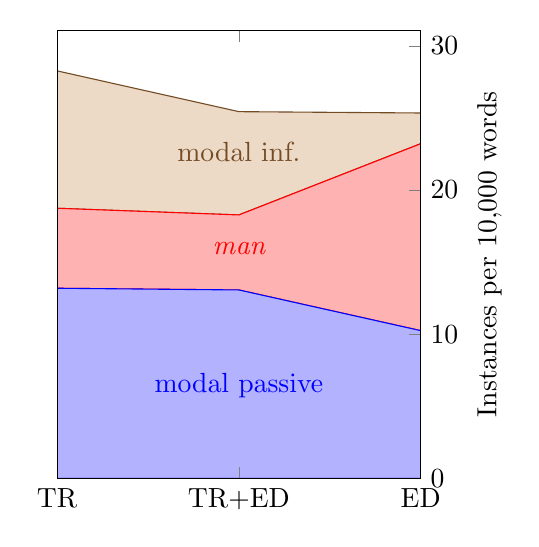
\begin{tikzpicture}
      \begin{axis}[
        width=62mm,
        height=207pt,
        stack plots=y,
        area style,ytick pos=right,
        symbolic x coords={TR,TR+ED,ED},
        xtick=data,ymin=0,
        ylabel={Instances per 10,000 words},
        enlarge x limits=false,
        legend pos=south west,
        ]
        \addplot
        %[black,fill=black!15!white]
        coordinates
        {(TR,13.1881) (TR+ED,13.0694) (ED,10.2485)}
        node[below,
        %black
        ] at (axis cs:TR+ED,8) {modal passive}
        \closedcycle;
        \addplot
        %[black,fill=black!30!white]
        coordinates
        {(TR,5.5470) (TR+ED,5.2016) (ED,12.9649)}
        node[below,
        %black
        ] at (axis cs:TR+ED,17) {\itshape man}
        \closedcycle;
        \addplot
        %[black,fill=black!50!white]
        coordinates
        {(TR,9.5278) (TR+ED,7.1628) (ED,2.1276)}
        node[below,
        %black
        ] at (axis cs:TR+ED,24) {modal inf.}
        \closedcycle;
      \end{axis}
    \end{tikzpicture}
  \end{minipage}%
  \caption{Left: Mean normalised frequency of passive alternatives ($F(2,78)=0.39,~p=.6784$); Right: Mean normalised frequencies of modal infinitives, \emph{man} and the modal passive.}\label{bisiada:fig:passalt}
\end{figure}

\noindent A closer look at the individual passive alternatives, however, reveals some differences between the translated and the non-translated texts. Both unedited and edited translations use \emph{man} statistically highly significantly less often than the non-translated texts ($F(2,78)=7.96,~p=.0007$), confirmed by a Kruskal-Wallis test ($H=9.01~(df=2),~p=.0111$). In the translations, \emph{man} occurs at a frequency of around 5 instances per 10,000 words, while in the non-translations, it occurs at around 13 instances per 10,000 words. A post-hoc Tukey test confirms that this is statistically significant at the $p<.01$ level.

At the same time, both unedited and edited translations use the modal infinitive statistically highly significantly ($F(2,78)=12.26,~p<.0001$) more often than non-translated texts (at the $p<.01$ level, according to the post-hoc Tukey test). That interpretation is confirmed by a Kruskal-Wallis test ($H=22.42~(df=2),~p<.0001$). Modal infinitives occur at a frequency of 2 instances per 10,000 words in non-translated texts, and at a frequency of 9.5 and 7 instances per 10,000 words in the manuscript and published translations, respectively. The data seem to indicate that editors have approximated the frequency of modal infinitives to that of non-translated texts, but the post-hoc Tukey test shows that the difference between the unedited and edited translations is statistically insignificant.

\subsubsection{Degree of unconventional language use}

Translators have been claimed to be more conservative in their language use than authors of non-translated texts \parencite[242]{berfer11}. \textcite{kruger12} conducts her analysis by searching for hapax legomena (words that occur only once in a text) and then filtering out \enquote{lexicalised} words by using the spell checker and online dictionary in Microsoft Word.

That seems like a somewhat unconvincing method to decide which words count as lexicalised. Some words may be used regularly, but may not occur in a dictionary and thus would not count as lexicalised. \ili{German} has extensive means of compounding, making it even easier to coin new words. A further problem with using hapax legomena as a tool for analysing idiosyncracy of the lexis is that even the most unconventional or innovative words will not appear in the analysis if they are used a second time somewhere in the text.

Nevertheless, the analysis presented here also takes the initial step of isolating hapax legomena using AntConc. From the resulting lists, words that feature in the Hunspell dictionary\footnote{Available at: \url{http://hunspell.sourceforge.net/}}, abbreviations, web addresses, proper names and untranslated job titles have been filtered out. I have only considered English words as loan words if they were found in the text \enquote{as is}, that is without quotation marks or explanations. Like the lexicalisation issue, the question of whether or not something is a loan word is difficult to answer \parencite{heller02}. I will not pursue the notion of lexicalisation any further at this point.

\newpage 
A seminal study on lexical creativity in translation is \textcite{kenny01}. Based on her method, I have analysed the remaining words based on their frequency in the \emph{Deutscher Wortschatz} reference corpus \parencite{quaetal13} from the Leipzig Corpora Collection (see Section~\ref{bisiada:sec:linadv}). For the present purposes, I have reduced the list to lemmas in the frequency classes 18 or above, which means they are outside the 200,000 most frequent words in \ili{German}.

Even with those parameters, the methodology remains somewhat problematic. Technical terms that are not in the dictionary might be infrequent in the reference corpus and thus be considered idiosyncratic language use. However, overall, the method does what it should by measuring the different frequencies with which unconventional words are used in the texts.

Keeping the mentioned drawbacks in mind, the analysis shows quite clearly that non-translated articles make more use of unconventional or less established words than the translated texts (Figure~\ref{bisiada:fig:lexic}). The difference is most pronounced in the case of lexical items that are not attested in the Leipzig corpus, which occur at a frequency of less than 5 instances per 10,000 words in the translated texts, but at a frequency of 18.5 instances per 10,000 words in the non-translated articles. The rather large error bars for the non-translated texts indicate that the actual values depend largely on the individual style of the author.

A further interesting aspect is that unattested lexical items and those at frequency classes 21--24 occur less frequently in the edited translations than in the manuscript ones. That seems to indicate that editors attempt to make the text more conservative by removing unconventional words.

\begin{figure}
  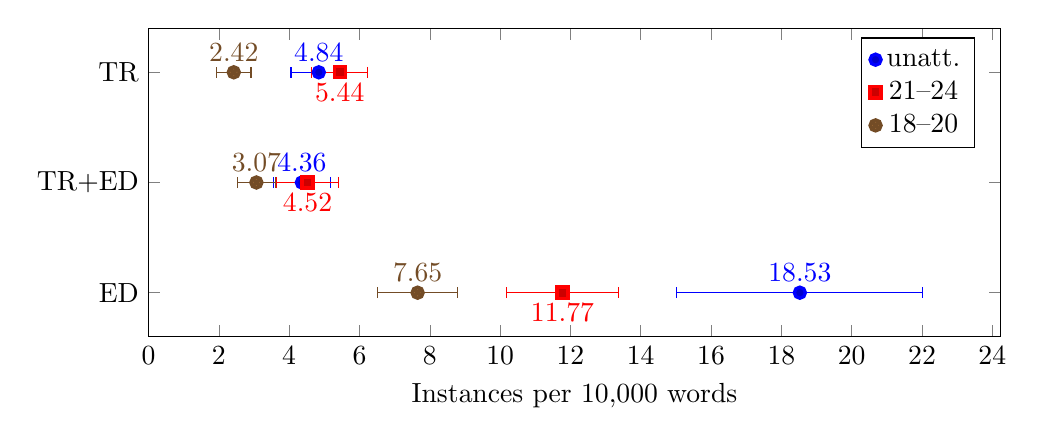
\begin{tikzpicture}
    \begin{axis}[
      height=55mm,width=124mm,
      symbolic y coords={ED,TR+ED,TR},
      ytick=data,enlarge y limits=0.2,xmin=0,
      nodes near coords,nodes near coords align={vertical},
      xlabel={Instances per 10,000 words},
      legend pos=north east,
      every axis plot/.append style={
        only marks,very thick,
        point meta=x,
      }
      ]
      \addplot+[error bars/.cd,x dir=both,x explicit]
      coordinates {
        (4.8429,TR)     +- (0.7893,0)
        (4.3613,TR+ED)  +- (0.8093,0)
        (18.5252,ED)    +- (3.5009,0)
      };
      \addlegendentry{unatt.}
      \addplot+[nodes near coords align={anchor=north},error bars/.cd,x dir=both,x explicit]
      coordinates {
        (5.4386,TR)     +- (0.7983,0)
        (4.5233,TR+ED)  +- (0.8757,0)
        (11.7738,ED)    +- (1.5976,0)
      };
      \addlegendentry{21--24}
      \addplot+[error bars/.cd,x dir=both,x explicit]
      coordinates {
        (2.4248,TR)     +- (0.4902,0)
        (3.0679,TR+ED)  +- (0.5463,0)
        (7.6535,ED)     +- (1.1292,0)
      };
      \addlegendentry{18--20}
    \end{axis}
  \end{tikzpicture}
  \caption{Mean normalised frequency of hapax legomena, unattested in the Leipzig corpus ($F(2,78)=14.34,~p<.0001$), at frequency classes 21--24 ($F(2,78)=11.82,~p<.0001$) and 18--20 ($F(2,78)=13.45,~p<.0001$)}\label{bisiada:fig:lexic}
\end{figure}

\newpage
The difference according to the ANOVA is highly significant for all three levels of frequency in the Leipzig corpus. It is confirmed by the Kruskal-Wallis test ($H=17.01~(df=2),~p<.0001$ for unattested words, $H=15.92~(df=2),~p<.0001$ for the frequency class 21--24 and $H=16.22~(df=2),~p<.0001$ for the frequency class 18--20). A post-hoc Tukey test shows that while the difference between translations and non-translations is significant at the $p<.01$ level in all three cases, there is no statistically significant difference between edited and unedited translations.

Nevertheless, with regard to the unattested words and those in the frequency classes of 21--24, there are fewer instances per 10,000 words in the edited translations compared to the unedited translations. Although that difference is not statistically significant according to the post-hoc Tukey test, it may still indicate that editors think more conservatively when it comes to \isi{editing} translations, whereas they leave more room for creativity to authors of non-translated texts. That is why it is only in non-translated texts that we find coinages and innovative compounds such as \emph{Gedankenwerker} (`thought worker'), \emph{glatterklären} (`smooth something out by explanation'), \emph{Abwarter} (`someone who hangs back and waits'), \emph{Lächelanordnungen} (`orders to smile') and \emph{lebenssprühend} (`sparking with life').

\subsubsection{Frequency of lexical bundles}

Kruger argues that the usage of lexical bundles, \enquote{\enquote{prefabricated}, conventionalised language unit[s]} is \textcquote[365]{kruger12}{indicative of more normalised or conservative language use}. Adopting her method to study lexical bundles, I have created a list of the most common trigrams in each corpus. Trigrams that occurred with a frequency of less than 0.01\% in each subcorpus were removed. Proper nouns such as \emph{Harvard Business School} and subject-specific trigrams such as \emph{Triple Bottom Line} were also removed.

Unlike Kruger, I have not removed individual subject-specific words. Given the fact that all texts form part of the same genre, I see no reason to exclude trigrams that contain subject-specific words, as they may be part of the particular jargon or conventionalised discourse of that language community. As a result, the list of the 28 trigrams that are investigated in this section (see Table~\ref{bisiada:tab:tgrtab}) contains some less general trigrams than the one used by \textcite[365]{kruger12}.

\begin{table}
  \caption{Trigrams selected for investigation}\label{bisiada:tab:tgrtab}
  \begin{tabular}{ll}
    \lsptoprule
    \emph{in der Regel} `normally'                      & \emph{nicht nur} \textsc{art} `not just the'\\
    \emph{bei der Entwicklung} `while developing'       & \emph{bei der Arbeit} `at work'\\
    \emph{für das Unternehmen}  `for the company'       & \emph{in den letzten} `in the last'\\
    \emph{auf diese Weise} `in this way'                & \emph{aus diesem Grund} `for this reason'\\
    \emph{eine Reihe von} `a range of'                  & \emph{in den vergangenen} `in the past'\\
    \emph{die Zahl der} `the number of'                 & \emph{dass die Mitarbeiter} `that the staff'\\
    \emph{davon überzeugt, dass} `convinced that'       & \emph{in der Praxis} `practically'\\
    \emph{zum Beispiel} \textsc{art} `for example the'  & \emph{in der Lage} `able to'\\
    \emph{handelt es sich} `is about'                   & \emph{für den Kunden} `for the customer'\\
    \emph{die Mitarbeiter, die} `employees who'         & \emph{in Bezug auf} `in relation to'\\
    \emph{Auswirkungen auf} \textsc{art} `effects on'   & \emph{dass sich} \textsc{art} `that \textsc{refl}'\\
    \emph{für den Erfolg} `for success'                 & \emph{in diesem Fall} `in this case'\\
    \emph{mit ihren Mitarbeitern} `with its staff'      & \emph{Art und Weise} `way'\\
    \emph{im Laufe der} `over the course of'            & \emph{sich heraus, dass} `turns out that'\\
    \lspbottomrule
  \end{tabular}
\end{table}

The ANOVA reveals that there is a highly significant difference among the three subcorpora (see Figure~\ref{bisiada:fig:trigr}), which is confirmed by a Kruskal-Wallis test ($H=23.02~(df=2),~p<.0001$). It is evident from the figure that this difference is found between the non-translations and the two subcorpora of manuscript and published translations. In the latter, the investigated trigrams occur with rather similar frequencies of 3.5 and 3.6 instances per 1,000 words, while in the non-translated articles, they only occur at a frequency of 2.1 instances per 1,000 words. The post-hoc Tukey test confirms that this is a significant difference at the $p<.01$ level.

\begin{figure}
  \begin{tikzpicture}
    \begin{axis}[anova,ylabel={Instances per 1,000 words}]
      \addplot table[row sep=\\,y error=error,]
      {
      sample  value   error   anchor\\
      TR    3.6295  0.2053  {south west}\\
      TR+ED 3.5307  0.2451  {south west}\\
      ED    2.1111  0.1898  {north east}\\
      };
    \end{axis}
  \end{tikzpicture}
  \caption{Mean normalised frequency of trigrams ($F(2,78)=15.66,~p<.0001$)}\label{bisiada:fig:trigr}
\end{figure}

Based on the higher occurrence of common trigrams in the translated texts, it would seem that translators are more conservative in their language use, and that editors have not intervened in this respect. The analysis of selected trigrams applied here is limited to analysing the frequency of specific tokens, while \textcquote[384]{kruger12}{obscuring differences in terms of the number of bundle types in the three subcorpora}.

Thus, in order to strengthen the analysis of conservative or normalised language use in the present corpus, I have conducted a general collocational analysis. As different measures of collocational association tend to produce different types of associations, the strength of an analysis is increased by studying several measures of association \parencite[373]{barber03}. The present analysis is therefore based on the log-likelihood and \isi{mutual information} \parencite[for more information on these measures, see][ch. 5.3--5.4]{mansch99}.

\noindent For this analysis, I have used Ted Pedersen's Ngram Statistics Package \parencite{banped03}.\footnote{Available at \url{http://ngram.sourceforge.net}} Based on the method used by \textcite{barber03}, the percentages of trigrams at or above certain cut-off points were compared for each subcorpus. High association scores mean a higher degree of collocational expression and thus, according to the present hypothesis, a more normalised language use.

For the log-likelihood ratio, three cut-off points were chosen. Log-likelihood ratios can be looked up directly in the table of the $\chi$\textsuperscript{2} distribution \parencite[174]{mansch99}. Thus, the cut-off points chosen here are the critical values 18.47, 23.51 and 28.47 given in the table for four degrees of freedom,\footnote{There are four degree of freedom because there are four independent values: one per word in the trigram and the total number of trigrams.} which correspond to the confidence levels $\alpha=0.001$, $\alpha=0.0001$ and $\alpha=0.00001$.

For the \isi{mutual information} score, \textcite{barber03} use pointwise \isi{mutual information}. In my case, the results produced by a pointwise \isi{mutual information} analysis did not seem to be a good representation of actual trigrams in the corpus \parencite[see][178--183 for a criticism of pointwise \isi{mutual information} as a measure of association]{mansch99}, so I chose to calculate the (true) \isi{mutual information} score instead. As the scores are all quite low, there is only one cut-off point at a \isi{mutual information} score of 0.01.

The results are shown in Figure~\ref{bisiada:fig:trigr-as}. Surprisingly, the mean percentage of trigrams with a log-likelihood ratio at or above the specified cut-off points is higher in the non-translated texts than in the translated texts, though the difference seems to disappear if the cut-off point is set to a higher value and thus a stricter confidence level. The non-translated texts also have a higher \isi{mutual information} score than the translations.

\begin{figure}[t]
  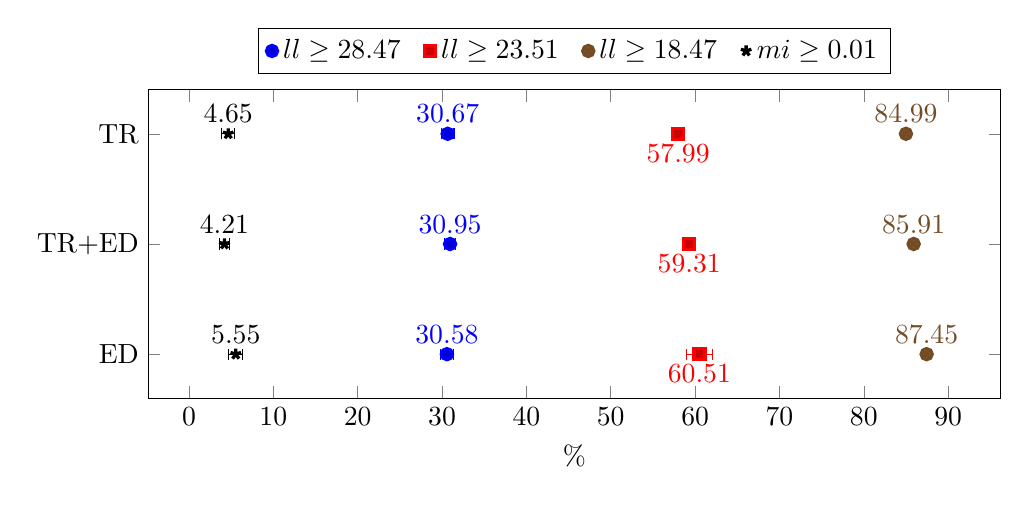
\begin{tikzpicture}
    \begin{axis}[%anova,
      height=55mm,width=124mm,
      symbolic y coords={ED,TR+ED,TR},
      ytick=data,enlarge y limits=0.2,
      nodes near coords,nodes near coords align={vertical},
      legend style={at={(0.5,1.05)},anchor=south},
      legend columns=4,
      xlabel={\%},
      every axis plot/.append style={
        only marks,very thick,
        point meta=x,
      }
      ]
      \addplot+[error bars/.cd,x dir=both,x explicit]
      coordinates {
        (30.6707,TR)    +- (0.7541,0)
        (30.9522,TR+ED) +- (0.621,0)
        (30.5807,ED)    +- (0.7901,0)
      };
      \addlegendentry{$\text{ll}\geq28.47~~$}
      \addplot+[nodes near coords align={anchor=north},error bars/.cd,x dir=both,x explicit]
      coordinates {
        (57.9919,TR)    +- (0.6488,0)
        (59.3078,TR+ED) +- (0.4916,0)
        (60.507,ED)     +- (1.5286,0)
      };
      \addlegendentry{$\text{ll}\geq23.51~~$}
      \addplot+[error bars/.cd,x dir=both,x explicit]
      coordinates {
        (84.9948,TR)    +- (0.3992,0)
        (85.9078,TR+ED) +- (0.2901,0)
        (87.447,ED)     +- (0.3237,0)
      };
      \addlegendentry{$\text{ll}\geq18.47~~$}
      \addplot+[error bars/.cd,x dir=both,x explicit]
      coordinates {
        (4.6533,TR)     +- (0.7785,0)
        (4.2104,TR+ED)  +- (0.5867,0)
        (5.5507,ED)     +- (0.8116,0)
      };
      \addlegendentry{$\text{mi}\geq0.01$}
    \end{axis}
  \end{tikzpicture}
  \caption{Mean percentages of trigrams at or above the log-likelihood ratios 28.47 ($F(2,78)=0.07,~p=.9325$), 23.51 ($F(2,78)=5.04,~p=.0087$), 18.47 ($F(2,78)=13.23,~p<.0001$), and the mutual information score 0.01 ($F(2,78)=0.87,~p=.423$)}\label{bisiada:fig:trigr-as}
\end{figure}

\noindent The statistical tests confirm this observation. For the lowest cut-off point in the log-likelihood ratio, a score of 18.47, the ANOVA reports a highly statistically significant difference, confirmed by the Kruskal-Wallis test ($H=22.48~(df=2),~p<.0001$). The post-hoc Tukey test confirms that the percentage value of the non-translations is significantly higher than those of both manuscript and published translations at the $p<.01$ level.

For the next cut-off point, 23.51, the ANOVA shows a highly statistically significant difference, confirmed by the Kruskal-Wallis test ($H=8.53~(df=2),~p=.0141$). The post-hoc Tukey test reveals that the value of the non-translations is still significantly higher than that of manuscript translations at the $p<.01$ level, but not higher than that of edited translations. Also, there is no statistically significant difference between the two translated subcorpora.

Regarding the highest cut-off point in the log-likelihood ratio, a score of 28.47, there is no significant difference between the corpora. In the case of the \isi{mutual information} score, the ANOVA yields no significant difference either.

The results from the collocational analysis support the tendency observed so far in this section, that translating creates a greater similarity between texts than \isi{editing}. However, the results do not seem to confirm the hypothesis that translations use more collocational and thus normalised language, which was supported by the finding that translations use a set of very frequent trigrams more often than non-translations. A technical explanation may be that the values yielded by the lower cut-off points are simply not very meaningful; after all, at the highest cut-off point, the difference disappears.

Another possible explanation might be that the use of translation memories favours a set of fixed, recurring phrases which are then used with a high frequency in the translations. That would explain why the set of trigrams chosen above occurs more often in translated than in non-translated texts. The latter, however, make more use of collocational language in general, which provides evidence against the hypothesis that translators use more normalised language. An explanation for this might be that writers have greater lexical freedom, and thus adopt specific collocations while translators are bound to the source text and thus less free in their language use.

To sum up this section, the analysis of unconventional language use and of lexical bundles argues that there are greater differences between the two translated texts on the one hand and the non-translated articles on the other. In other words, the \isi{editing} process does not significantly change the features of the language of translation, which make the text differ from a non-translated text.

%%%%%%%%%%%%%%%%%%%%%%%%%%%%%%%%%%%%%%%%%%%%%%%%%%%%%%%%%%%%%%%%%%%%%%%%%%%%%%%%%%%%%
\subsection{Simplification}\label{bisiada:sec:simp}
%%%%%%%%%%%%%%%%%%%%%%%%%%%%%%%%%%%%%%%%%%%%%%%%%%%%%%%%%%%%%%%%%%%%%%%%%%%%%%%%%%%%%

\subsubsection{Lexical diversity}

For the analysis of \isi{lexical diversity}, \textcite{kruger12} uses the standardised type-token ratio. I use the moving-average type-token ratio (MATTR) instead, which is a more robust measure of \isi{lexical diversity} than the STTR because it is not affected by text length and takes into account changes within the text \parencite[96]{covmcf10}. I adopt a 500 word window as suggested for stylometric analyses by the authors \parencite[97]{covmcf10}. The MATTR was calculated using the R package koRpus by Meik Michalke.\footnote{\url{http://reaktanz.de/?c=hacking&s=koRpus}}

The ANOVA yields a highly statistically significant difference between the corpora (see Figure~\ref{bisiada:fig:mattr}). The distribution of the TR+ED subcorpus is skewed, but the Kruskal Wallis test confirms a highly statistically significant difference among the corpora ($H=18.88~(df=2),~p<.0001$). A post-hoc Tukey test reveals that the mean MATTR of the manuscript translations is significantly lower at the ($p<.01$) level than the mean MATTRs of both edited texts. The edited texts among themselves do not show a significant difference in mean MATTR.

\begin{figure}
  \begin{tikzpicture}
    \begin{axis}[anova,ylabel={MATTR}]
      \addplot table[row sep=\\,y error=error,]
      {
      sample  value   error   anchor\\
      TR    0.8100  0.0030  {north west}\\
      TR+ED 0.8207  0.0029  {south east}\\
      ED    0.8285  0.0026  {north east}\\
      };
    \end{axis}
  \end{tikzpicture}
  \caption{Moving-average type-token ratio ($F(2,78)=10.76,~p=.0018$)}\label{bisiada:fig:mattr}
\end{figure}

\noindent The findings argue that the manuscript translations are lexically less diverse than both non-translations and their published versions, which shows that the editors have intervened significantly to increase \isi{lexical diversity}. The assumption that translations have a less varied vocabulary and are therefore simpler is supported. This analysis exemplifies the value of comparing manuscript and edited translations, as in a traditional corpus design, the fact that the actual translations have a much lower \isi{lexical diversity} value would not have surfaced.

\subsubsection{Word and sentence length}

Word and sentence length were also calculated with the R package koRpus. Word length operationalises simplicity because more specific or formal words are usually longer while more frequent words are shorter \parencites[366]{kruger12}{biber91}, which seems especially true in the case of \ili{German} \parencite[46]{benetal04}.

Sentence length is usually considered to be an indicator of simplification, as sentences in translated texts tend to be shorter \parencite{laviosa02}. As longer sentences are deemed harder to understand \parencite[though this may be problematic generalisation; see the discussion in][165--169]{Bisiada2013} it is assumed that translators split sentences to improve readability \parencites[212]{vinhan05}[21]{bisiada14}. Simplification as a translation universal may therefore be operationalised by measuring sentence length.
% update your page number once the paper finally appears in an issue (if ever...)

In terms of the mean word length, the ANOVA reports no statistically significant difference between the three subcorpora (see the graph on the left in Figure~\ref{bisiada:fig:mwsl}).

\begin{figure}
  \begin{minipage}{0.5\textwidth}
    \begin{tikzpicture}
      \begin{axis}[anova,height=207pt,width=63mm,ylabel={Letters}]
        \addplot table[row sep=\\,y error=error,]
        {
        sample  value   error   anchor\\
        TR    6.133   0.0590  {south west}\\
        TR+ED 6.147   0.0564  {north east}\\
        ED    6.144   0.0590  {north east}\\
        };
      \end{axis}
    \end{tikzpicture}
    \end{minipage}%
    \begin{minipage}{0.5\textwidth}%
      \begin{tikzpicture}
      \begin{axis}[anova,height=207pt,width=65mm,ylabel={Words},ytick pos=right]
        \addplot table[row sep=\\,y error=error,]
        {
        sample  value   error   anchor\\
        TR    17.957  0.3941  {south west}\\
        TR+ED 16.679  0.3535  {north east}\\
        ED    15.909  0.2442  {north east}\\
        };
      \end{axis}
    \end{tikzpicture}
  \end{minipage}
  \caption{Left: Mean word length ($F(2,78)=0.01,~p=.9901$); Right: Mean sentence length ($F(2,78)=9.44,~p=.0002$)}\label{bisiada:fig:mwsl}
\end{figure}

\noindent For the mean sentence lengths in the subcorpora, contrary to what is usually assumed, it seems that the sentences in the manuscript translations are longer than those in the edited translations, and even more so than those in the non-translations (see the right graph in Figure~\ref{bisiada:fig:mwsl}).

The difference is highly statistically significant according to the ANOVA, and confirmed by the Kruskal-Wallis test ($H=20.64~(df=2),~p<.0001$). A post-hoc Tukey test shows that the manuscript translations differ from both edited texts. Sentences in manuscript translations are highly significantly ($p<.01$) longer than in the non-translations and significantly ($p<.05$) longer than in the published translations. The two edited texts do not exhibit a statistically significant difference to each other.

It appears that the editors have brought the translated texts closer to the average sentence length that is exhibited by the non-translated texts. An analysis of the manuscript non-translations would be useful here to see whether editors have shortened the sentences in those texts as well. The strong editorial influence with regard to sentence length further underlines the need to differentiate manuscripts from edited versions when making statements about the features of translated language.

This section has produced results that contrast with those from the two sections on \isi{explicitation} and normalisation\slash conservatism in that there seem to be greater similarities between the edited translations and the non-translated articles. This suggests that, with regard to simplification, the \isi{editing} process has rendered the language in the translated texts more similar to that encountered in the non-translated texts.

%%%%%%%%%%%%%%%%%%%%%%%%%%%%%%%%%%%%%%%%%%%%%%%%%%%%%%%%%%%%%%%%%%%%%%%%%%%%%%%%%%%%%
\section{Summary and discussion}\label{bisiada:sec:disc}
%%%%%%%%%%%%%%%%%%%%%%%%%%%%%%%%%%%%%%%%%%%%%%%%%%%%%%%%%%%%%%%%%%%%%%%%%%%%%%%%%%%%%

The analysis in this chapter has produced a large amount of data and claims which I hope will be checked and confirmed or rejected by other scholars, so that we discover more about the effect of \isi{editing} on translation. Table~\ref{bisiada:tab:sum} provides an overview of the mean values that have resulted from the analysis in this chapter. For completeness' sake, standard deviations are also supplied in brackets.

\begin{table}[b]
  \caption{Overview of values with standard deviation in brackets}\label{bisiada:tab:sum}
  \begin{tabular}{ld{2}@{ }d{2}d{2}@{ }d{2}d{2}@{ }d{2}r}
  \lsptoprule
  Variable & \multicolumn{2}{c}{TR} & \multicolumn{2}{c}{TR+ED} & \multicolumn{2}{c}{ED} & p\\
  \midrule
  \emph{dass} present       & 17.48 & (12.68)  & 17.41 & (11.03) & \cellcolor{lsMidBlue!50}9.30 & \cellcolor{lsMidBlue!50}(6.33)  & <.01\\
  \emph{dass} absent        & 8.52  & (10.59)  & 9.47 & (7.60)  & 7.48              & (7.98)  & >.05\\
  PAV                       & 9.43  & (1.68)   & 9.45 & (1.74)  & 7.99              & (2.69)  & >.05\\
  Linking                   & 9.22  & (2.21)   & 9.21 & (2.65)  & 8.52              & (3.06)  & >.05\\
  Conj vs Prep              & 0.63  & (0.13)   & 0.68 & (0.11)  & 0.65              & (0.12)  & >.05\\
  \midrule
  Passive alt.              & 28.26 & (15.40)  & 25.43                   &(12.02)   & 25.34                     & (13.69)                     & >.05\\
  Unconv. (unatt.)          & 4.84  & (4.10)   & 4.36                    &(4.21)    & \cellcolor{lsMidBlue!50}18.53 & \cellcolor{lsMidBlue!50}(18.19) & <.01\\
  Unconv. (21--24)          & 5.44  & (4.15)   & 4.52                    &(4.55)    & \cellcolor{lsMidBlue!50}11.77 & \cellcolor{lsMidBlue!50}(8.30)  & <.01\\
  Unconv. (18--20)          & 2.42  & (2.55)   & 3.07                    &(2.84)    & \cellcolor{lsMidBlue!50}7.65  & \cellcolor{lsMidBlue!50}(5.87)  & <.01\\
  Trigrams                  & 3.62  & (1.07)   & 3.53                    &(1.27)    & \cellcolor{lsMidBlue!50}2.11  & \cellcolor{lsMidBlue!50}(0.99)  & <.01\\
  Trigr. (ll, cut-off low)  & 84.99 & (2.07)   & 85.91                   &(1.51)    & \cellcolor{lsMidOrange!50}87.45   & \cellcolor{lsMidOrange!50}(1.68)    & <.01\\
  Trigr. (ll, cut-off mid)  & 57.99 & (3.37)   & \cellcolor{lsMidOrange!30}59.31 & \cellcolor{lsMidOrange!30}(2.55)  & \cellcolor{lsMidOrange!50}60.51   & \cellcolor{lsMidOrange!50}(2.75)    & <.01\\
  Trigr. (ll, cut-off high) & 30.67 & (3.92)   & 30.95                   & (3.23)   & 30.58                     & (4.11)                      & >.05\\
  Trigr. (mi)               & 4.65  & (4.04)   & 4.21                    & (3.05)   & 5.55                      & (4.22)                      & >.05\\
  \midrule
  MATTR                     & \cellcolor{lsMidBlue!50}0.81 & \cellcolor{lsMidBlue!50}(0.02)  & 0.82                    & (0.02)                    & 0.83  & (0.01)  & <.01\\
  WL                        & 6.13                     & (0.31)                      & 6.15                    & (0.29)                    & 6.14  & (0.31)  & >.05\\
  SL                        & \cellcolor{lsMidOrange!50}17.96  & \cellcolor{lsMidOrange!50}(2.05)    & \cellcolor{lsMidOrange!30}16.68 & \cellcolor{lsMidOrange!30}(1.84)  & 15.91 & (1.27)  & <.01\\
  \lspbottomrule
  \end{tabular}
\end{table}

Cells in colour represent values that are different from the values of the other corpora. If the colour is blue, it means that the value behaves as expected under the universal in question; if the colour is orange, it means that the value runs counter to expectations and does not support the usual hypothesis attributed to that universal (the hypotheses attributed to each universal are discussed for each operationalisation in Sections~\ref{bisiada:sec:expl}, \ref{bisiada:sec:norm} and \ref{bisiada:sec:simp}). The lighter colour means that the difference is statistically significant and a darker colour means that the difference was shown to be highly statistically significant. Values in the colourless cells are not significantly different to each other.

In the case of \isi{explicitation}, most variables analysed here show no difference to each other, so that the features across the three subcorpora are mostly the same, except there are fewer explicitations using \emph{dass} clauses in the non-translated articles. The differences are thus restricted to cases of less economical surface realisation, a \enquote{borderline case} of \isi{explicitation} that may more usefully be considered as \textcquote[239]{krueger15}{expansion}. Alternatively, the more frequent presence of \emph{dass} in translated texts may be a sign of conservative language use if we accept the claim that a \ili{German} finite \emph{dass}-clause is preferred over a non-finite \isi{construction} \parencites[215]{fischer97}[337]{fischer13}, though this claim has not yet been backed up by evidence.

As the use of normalised or conservative language is concerned, the operationalisations analysed here suggest that there is a difference between translated and non-translated language. The latter makes more use of unconventional language and differs in the use of collocations. As regards the latter, it seems that translators use a set of recurring trigrams more frequently than writers of non-translated articles, but overall, the latter seem to use more collocational language.

In terms of the universal of simplification, differences have been observed between manuscript translations on the one hand and edited translations as well as non-translations on the other. This seems to show that editors' influence has been strongest in this respect, arguing for simplification to be an \isi{editing} universal. An explanation for this might be that simplification is operationalised by mainly quantitative features, which makes it easier for editors to change the text in order to approximate its language to the non-translated articles. More research on other genres and text types should test editors' influence on sentence length. This may explore the question of whether the finding that (published) translations have shorter sentences on average can actually be related to translated language, or whether it should instead be attributed to the influence of editors who try to improve the readability of a text.

As for the hypothesis of \isi{universals} of mediated discourse, the study produces little evidence in favour of \enquote{\isi{mediation} universals}. Verifying that theory in the present study would have required the data to show more similarities between the TR+ED and the ED subcorpora, and for there to be more differences between the TR and the TR+ED subcorpora.

Instead, and similarly to what was reported by \textcite{kruger12}, the \isi{editing} stage seems to have little effect on the features measured here. That does not mean that changes to the text are negligible, but rather that editors do not intervene in such a way to make the articles more like the non-translated articles. With regard to simplification, however, my findings differ from those reported in \textcite{kruger12}, as editors have made significant changes in this respect.

Based on the present findings, it could be argued that \isi{editing} is largely a simplifying activity, with editors trying to apply quantitative strategies to make the text more comprehensible \parencite[on this issue, see also][]{mueetal15}. The general direction of editorial behaviour seems to incorporate changes that are thought to \enquote{improve} the text from the editor's point of view, and mainly focus on superficially identifiable features such as shortening sentence length \parencite[on editorial sentence splitting in translation, see][]{bisiada14} or effecting lexical changes that lower the type token ratio. The editorial style of course depends to a great extent on genre. Texts edited for commercial publications need to be more reader-friendly than, say, reports or parliament communications. The \isi{editing} activity here is heavily guided by the in-house style guide, which does stipulate simple language \parencite[3]{bisiada14}.

From a practical perspective, the findings show that editors' intervention is restricted to three features: they make sentences shorter \parencite[by splitting them, as reported for \ili{German} in][]{bisiada14}, they increase \isi{lexical diversity} and they increase collocational language use to some extent. They also seem to reduce the frequency of alternative passive constructions, though the difference in this case is not statistically significant. I discuss this issue in more detail in a monograph currently in preparation.

With regard to the omission of \emph{dass} and the unconventional words, editors seem to have made the text more unlike the non-translated texts. While again the differences are not statistically significant, this may mean that when \isi{editing} translations, editors are actually more conservative and restrictive in terms of the non-standard expressions they let pass than when they are \isi{editing} non-translated articles. In this respect, translations may improve or at least be more consistent with non-translated articles if editors gave translators some more freedom and allowed more unconventional language use.

To empirically strengthen the discipline of translation studies, more transparent and replicable research is needed. I have tried to provide such a study in this chapter, and hope to have offered a range of avenues for further research. As was shown in this chapter, the study of \isi{editing} can greatly enhance our view of the \isi{translation process} by differentiating features that really are attributable to translation from those that are introduced by other agents who have influence on the text.

\section*{Acknowledgments}

This research was conducted as part of the project \emph{Evidencialidad y epistemicidad en textos de géneros discursivos evaluativos. Análisis contrastivo y traduccion} (ModevigTrad) [`Evidentiality and epistemicity in texts of evaluative discourse genres. Contrastive analysis and translation'], with reference number FFI2014-57313-P, funded by the \ili{Spanish} Ministerio de Economía y Competitividad.

This paper has benefitted from a discussion on Academia.edu, where I have made the manuscript available to invite criticism and suggestions from the scholarly community, with the aim of trialling a kind of \enquote{community peer review}. I would like to thank everyone who participated in this session, especially my colleagues Ralph Krüger, Ekaterina Lapshinova-Koltunski, Sofia Malamatidou, Timothy Huson and Gemma Andújar Moreno for their critical reading, suggestions and detailed feedback on this paper.

I~thank Michael Heinrichs at the translation company Rheinschrift for his efforts with the publishing company to allow me to obtain the manuscript translations for research purposes.

I~am equally indebted to the editors at the \emph{Harvard Business Manager}, especially Britta Domke, for their interest in my research and for giving me valuable insights into their workflow.

For all statistical calculations, I have used Richard Lowry's comprehensive yet accessible website VassarStats (\url{http://www.vassarstats.net}) and would like to thank him for making this excellent tool freely available.
% todo: before accepting the final version, repeat every single calculation and check every graph

\sloppy
\printbibliography[heading=subbibliography,notkeyword=this]
\end{document}
